% Provenance (never printed): NSI terminale project closing the year: "Bases de donnees" + "Algorithmique:
% algorithmes sur les graphes" + "Structures de donnees: interface et implementation, vocabulaire de la programmation
% objet" turned into one programming project. See sources/book2/BRIEFS.md.
\chapter{Project: A Route Planner}\label{ch:g12:project-route-planner}

A route planner answers one question: what is the fastest way from here to there? Behind the question sit three
pieces of this year's work. The map is data, kept in a \omterm{def:g12:relational-databases-sql:database}{database}; the roads form a \omterm{def:g10:graphs-first-look:graph}{graph}; and the answer is a shortest
path, found by \omterm{met:g12:graph-algorithms:dijkstra}{Dijkstra's algorithm}. This project joins the three into one program for the town of Brenmoor, the
invented town of the series, with a class that hides how it works and a small text interface in front of it.

\begin{omfigure}
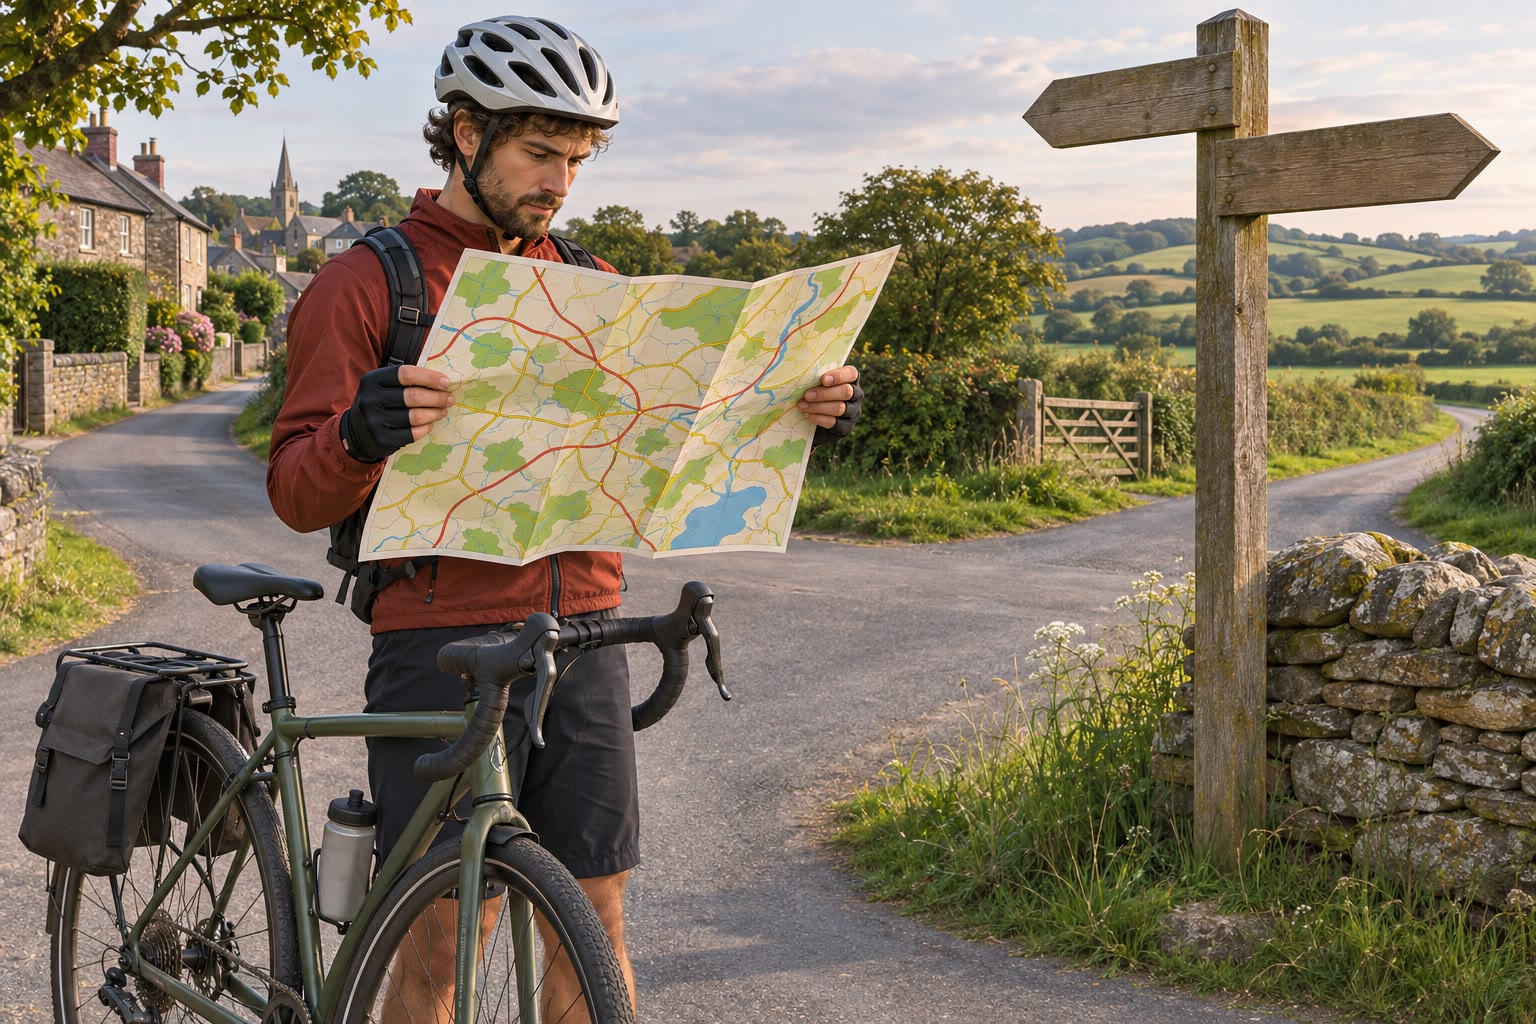
\includegraphics[width=0.5\linewidth]{images/book2/ai/g12-project-route-planner-cyclist.jpg}

{\small The question a route planner answers, asked the old way.}
\end{omfigure}

\begin{recall}
Tables, keys and \omterm{def:g12:relational-databases-sql:sql}{SQL} queries (chapter \ref{ch:g12:relational-databases-sql}). Directed and \omterm{def:g10:graphs-first-look:directed}{weighted graphs}
(chapter \ref{ch:g10:graphs-first-look}), and \omterm{met:g12:graph-algorithms:dijkstra}{Dijkstra's algorithm} with its parents (chapter
\ref{ch:g12:graph-algorithms}). Classes, methods and interfaces (chapters \ref{ch:g12:classes-and-objects} and
\ref{ch:g11:modules-and-interfaces}). \omterm{def:g10:specifications-and-tests:test-suite}{Test suites} with \code{unittest} (chapter \ref{ch:g10:specifications-and-tests}).
\end{recall}

\section{The specification}\label{sec:g12:project-route-planner:spec}

Write, in Python, a program that answers ``fastest route from place $A$ to place $B$'' in Brenmoor. The places and
roads are stored in an SQLite \omterm{def:g12:relational-databases-sql:database}{database} with keys and \omterm{def:g12:relational-databases-sql:schema}{integrity constraints}, filled from the town's tables. They are
loaded into a \omterm{def:g10:graphs-first-look:directed}{directed graph} whose arcs carry the travel time in seconds, computed from the length of each road and
its speed limit; a one-way road gives a single arc. \omterm{met:g12:graph-algorithms:dijkstra}{Dijkstra's algorithm} returns the route and its time. A class
\code{RoutePlanner} offers a documented interface: a route by time or by distance, a road closed and reopened, and an
error for a place that does not exist. A text menu lets a person use it, and a \omterm{def:g10:specifications-and-tests:test-suite}{test suite} checks every function.

The work goes in five milestones, each one runnable before the next starts. The town's tables are read with the
series' module \code{town}, which is imported and never changed.

\begin{omfigure}
\begin{tikzpicture}[box/.style={draw, rounded corners=2pt, minimum height=11mm, text width=24mm, align=center,
    font=\footnotesize}, ->, >=stealth]
  \node[box, fill=black!5] (csv) at (0,0) {town tables\\ \code{places}, \code{roads}};
  \node[box, fill=omDef!10] (db) at (3.4,0) {database\\ \code{db.py}};
  \node[box, fill=omMeth!12] (g) at (6.8,0) {graph\\ \code{graph.py}};
  \node[box, fill=omThm!10] (alg) at (10.2,0) {algorithm\\ \code{planner.py}};
  \node[box, fill=omDef!10] (ui) at (10.2,-2.2) {interface\\ \code{menu.py}};
  \node[box, fill=black!5] (user) at (6.8,-2.2) {a person\\ at the keyboard};
  \draw (csv) -- node[above, font=\scriptsize] {M1} (db);
  \draw (db) -- node[above, font=\scriptsize] {M2} (g);
  \draw (g) -- node[above, font=\scriptsize] {M3} (alg);
  \draw (alg) -- node[right, font=\scriptsize] {M4} (ui);
  \draw[<->] (ui) -- (user);
  \node[font=\scriptsize, text width=40mm, align=center] at (3.4,-2.2) {M5: tests of every box, and a measure
    over every pair of places};
\end{tikzpicture}

{\small The architecture. Each box is one module and one milestone; each arrow is the only way data passes from one
module to the next. The interface never sees the \omterm{def:g12:relational-databases-sql:database}{database}, and the algorithm never sees \omterm{def:g12:relational-databases-sql:sql}{SQL}.}
\end{omfigure}

\section{Milestone 1: the database}\label{sec:g12:project-route-planner:m1}

The planner keeps its own two tables, \code{place} and \code{road}, with the constraints that make bad data impossible
to store: every road starts and ends at a place that exists, has a positive length and a sensible speed limit, and
does not join a place to itself; no two places share a name, since the interface finds places by name.

\begin{omfigure}
\begin{tikzpicture}[font=\footnotesize]
  \node[draw, fill=omDef!8, inner sep=3pt] (place) at (0,0) {\begin{tabular}{l}
    \textbf{place}\\ \hline
    \code{place_id} \quad integer, primary key\\
    \code{name} \quad text, not null, unique\\
    \code{kind} \quad text, not null
  \end{tabular}};
  \node[draw, fill=omMeth!8, inner sep=3pt] (road) at (7.4,0) {\begin{tabular}{l}
    \textbf{road}\\ \hline
    \code{road_id} \quad integer, primary key\\
    \code{from_place} \quad references \code{place}\\
    \code{to_place} \quad references \code{place}\\
    \code{length_m} \quad integer $> 0$\\
    \code{speed_kmh} \quad integer from $10$ to $130$\\
    \code{one_way} \quad $0$ or $1$
  \end{tabular}};
  \draw[->, >=stealth, omThm, thick] ([yshift=3mm]road.west) -- node[above, font=\scriptsize] {\code{from_place}}
    ([yshift=3mm]place.east);
  \draw[->, >=stealth, omThm, thick] ([yshift=-3mm]road.west) -- node[below, font=\scriptsize] {\code{to_place}}
    ([yshift=-3mm]place.east);
  \node[font=\scriptsize, anchor=north] at (road.south) {and \code{from_place} $\ne$ \code{to_place}};
\end{tikzpicture}

{\small The schema of the planner's \omterm{def:g12:relational-databases-sql:database}{database}. Each road refers to two places through
two \omterm{def:g12:relational-databases-sql:keys}{foreign keys}; the checks on the right are the \omterm{def:g12:relational-databases-sql:schema}{integrity constraints} that SQLite enforces at every insertion.}
\end{omfigure}

\omcode{code/grade-12/14-project-route-planner/listings/db.py}{1}{36}{Milestone 1: the schema, and a \omterm{def:g12:relational-databases-sql:database}{database} filled
from the town's tables.}\label{lst:g12:project-route-planner:db}

SQLite checks \omterm{def:g12:relational-databases-sql:keys}{foreign keys} only when asked, with \code{PRAGMA foreign_keys = ON}, once per connection. The first run
counts the rows, shows the one-way road and the speed limits, and then tries three wrong insertions.

\omcode{code/grade-12/14-project-route-planner/listings/run_m1.py}{1}{19}{Milestone 1: counting, and three insertions
that the constraints must refuse.}\label{lst:g12:project-route-planner:m1}

\omoutput{code/grade-12/14-project-route-planner/outputs/run_m1.txt}{$30$ places, $53$ roads, one of them one-way;
each wrong row is refused with the name of the rule it breaks.}\label{out:g12:project-route-planner:m1}

The town's own tables, \code{places} and \code{roads}, carry the same columns and the coordinates of each place in
metres. Plain \omterm{def:g12:relational-databases-sql:sql}{SQL} already answers questions about the map, before any \omterm{def:g10:graphs-first-look:graph}{graph} exists.

\omcode{code/grade-12/14-project-route-planner/listings/queries.sql}{1}{8}{Three questions to the town's tables: the
commonest kinds of place, the longest roads, and the total length.}\label{lst:g12:project-route-planner:queries}

\omoutput{code/grade-12/14-project-route-planner/outputs/queries.txt}{The longest road, $1830$ metres, is also a slow
one: $30$ km/h.}\label{out:g12:project-route-planner:queries}

\section{Milestone 2: the graph}\label{sec:g12:project-route-planner:m2}

The roads become arcs. A road of length $\ell$ metres with a speed limit of $v$ km/h takes $\ell / (v / 3.6) = 3.6\,
\ell / v$ seconds, since $1$ km/h is $1000 / 3600$ metres per second. The cost is rounded to the second, so that every
time printed is a whole number.

\omcode{code/grade-12/14-project-route-planner/listings/graph.py}{1}{35}{Milestone 2: the travel time of a road, and a
class for a \omterm{def:g10:graphs-first-look:directed}{directed graph} with costs.}\label{lst:g12:project-route-planner:graph}

The class keeps a dictionary of dictionaries, the \omterm{def:g12:graph-algorithms:adjacency-list}{adjacency lists} of chapter \ref{ch:g12:graph-algorithms} with a cost
on each arc. The method \code{reachable} is a breadth-first search: it checks that the town is connected, in the
directed sense, from every place.

\omcode{code/grade-12/14-project-route-planner/listings/graph.py}{37}{54}{Milestone 2: arcs without their reverse, and
the \omterm{def:g10:graphs-first-look:graph}{graph} read from the \omterm{def:g12:relational-databases-sql:database}{database}, by time or by distance.}\label{lst:g12:project-route-planner:from-db}

\omcode{code/grade-12/14-project-route-planner/listings/run_m2.py}{1}{12}{Milestone 2: the checks of the
\omterm{def:g10:graphs-first-look:graph}{graph}.}\label{lst:g12:project-route-planner:m2}

\omoutput{code/grade-12/14-project-route-planner/outputs/run_m2.txt}{$2 \times 52 + 1 = 105$ arcs, every place
reaches every other, and only the arc $1 \to 3$ has no reverse.}\label{out:g12:project-route-planner:m2}

The three successors of the Station show the point of travel times: River Park and Hill Park, at $680$ and $690$
metres on roads at $70$ km/h, are $35$ seconds away, while the Town Hall, at $1000$ metres on a road at $30$ km/h, is
$120$ seconds away.

\section{Milestone 3: shortest routes}\label{sec:g12:project-route-planner:m3}

\omterm{met:g12:graph-algorithms:dijkstra}{Dijkstra's algorithm}, as in chapter \ref{ch:g12:graph-algorithms}, finishes at each step the unfinished vertex with
the smallest tentative cost, found by a scan, and records the parent of each vertex it improves. Following the parents
back from the target and reversing gives the route.

\omcode{code/grade-12/14-project-route-planner/listings/planner.py}{1}{23}{Milestone 3: \omterm{met:g12:graph-algorithms:dijkstra}{Dijkstra's algorithm} on a
\code{Graph}, and the route rebuilt from the parents.}\label{lst:g12:project-route-planner:dijkstra}

The class of the next milestone wraps these two functions; the first run uses it already, to compare the two criteria
and the two directions of the one-way road.

\omcode{code/grade-12/14-project-route-planner/listings/run_m3.py}{1}{13}{Milestone 3: by time and by distance, and
both ways between the Town Square and the Library.}\label{lst:g12:project-route-planner:m3}

\omoutput{code/grade-12/14-project-route-planner/outputs/run_m3.txt}{The two criteria can agree, or not: the shortest
road from the Allotments is not the fastest.}\label{out:g12:project-route-planner:m3}

From the Allotments to the Sports Hall the direct road is $1200$ metres at $50$ km/h, $86$ seconds; through the
College it is $180$ metres longer, on two roads at $70$ km/h, and takes $71$ seconds. The criterion is part of the
question: ``shortest'' and ``fastest'' are different \omterm{def:g10:graphs-first-look:graph}{graphs} on the same roads. And the one-way road makes the town
lopsided: $98$ seconds from the Town Square to the Library, $204$ seconds back, through the Garden Centre.

\begin{omfigure}
\begin{tikzpicture}
\begin{axis}[omrecord, width=10.5cm, height=8.8cm, xlabel={$x$ (km)}, ylabel={$y$ (km)}, xmin=-0.2, xmax=6, ymin=-0.2,
    ymax=5.1, axis equal image, grid=none]
  \addplot[black!25, line width=0.6pt] table[x=x, y=y]{code/grade-12/14-project-route-planner/figures/map_roads.dat};
  \addplot[omThm, line width=1.6pt] table[x=x, y=y]{code/grade-12/14-project-route-planner/figures/map_route.dat};
  \addplot[only marks, mark=*, mark size=1.5pt, omDef, nodes near coords, point meta=explicit symbolic,
    nodes near coords style={font=\tiny, black!60, anchor=south west, inner sep=1pt}]
    table[x=x, y=y, meta=id]{code/grade-12/14-project-route-planner/figures/map_places.dat};
  \node[font=\scriptsize, anchor=north] at (axis cs:1.217,0.70) {Old Mill};
  \node[font=\scriptsize, anchor=south] at (axis cs:5.28,3.64) {Post Office};
  \node[font=\scriptsize, anchor=north] at (axis cs:2.301,2.80) {Station};
\end{axis}
\end{tikzpicture}

{\small The town's $53$ roads (grey) drawn from the coordinates of the $30$ places, numbered by their
\code{place_id}, and in red the slowest of all fastest routes, from the Old Mill to the Post Office, as the planner
computes it (\code{figures/route_map.py}).}
\end{omfigure}

\section{Milestone 4: the interface}\label{sec:g12:project-route-planner:m4}

The class \code{RoutePlanner} is what the rest of the program sees. Its user names places and roads; the identifiers,
the \omterm{def:g10:graphs-first-look:graph}{graph} and the algorithm stay inside. A wrong name raises \code{ValueError} with a message, so that the menu can say
what went wrong instead of stopping.

\omcode{code/grade-12/14-project-route-planner/listings/planner.py}{26}{59}{Milestone 4: the class \code{RoutePlanner}
and its five methods.}\label{lst:g12:project-route-planner:class}

\begin{omfigure}
\begin{tikzpicture}[font=\footnotesize]
  \node[draw, fill=omThm!8, inner sep=3pt] (rp) at (0,0) {\begin{tabular}{l}
    \textbf{RoutePlanner}\\ \hline
    \code{conn}: the database\\
    \code{names}, \code{ids}: id $\leftrightarrow$ name\\
    \code{closed}: set of road numbers\\ \hline
    \code{place_id(name)}\\
    \code{route(start, end, criterion)}\\
    \code{cost_of(path, criterion)}\\
    \code{close_road(road_id)}\\
    \code{reopen_road(road_id)}
  \end{tabular}};
  \node[draw, fill=omMeth!8, inner sep=3pt] (g) at (8.2,0) {\begin{tabular}{l}
    \textbf{Graph}\\ \hline
    \code{arcs}: vertex $\to$ \{successor: cost\}\\ \hline
    \code{add_vertex(v)}, \code{add_arc(u, v, cost)}\\
    \code{successors(u)}, \code{arc_count()}\\
    \code{reachable(start)}\\
    \code{one_way_arcs()}
  \end{tabular}};
  \draw[->, >=stealth, dashed] (rp.east) -- node[above, font=\scriptsize, align=center] {builds one\\ per question}
    (g.west);
  \node[font=\scriptsize, anchor=north] at (g.south) {built by
    \code{from_database(conn, criterion, closed)}};
\end{tikzpicture}

{\small The two classes: name, then attributes, then methods. \code{RoutePlanner} builds a \code{Graph} for each
question, from the \omterm{def:g12:relational-databases-sql:database}{database} and the set of closed roads, and passes it to \code{dijkstra}.}
\end{omfigure}

Building the \omterm{def:g10:graphs-first-look:graph}{graph} again for each question costs a few hundred operations here; it keeps the class simple, since a
closed road then needs no change to any \omterm{def:g10:graphs-first-look:graph}{graph}. Exercise \ref{exo:g12:project-route-planner:9} counts the cost of the
whole town.

The menu reads a choice, then what that choice needs, and prints the answer in minutes and seconds. For the run below
its input comes from the file \code{menu.stdin}, one line per answer: a route, a misspelt name, road $2$ closed, the
same route again, a wrong choice, and the end.

\omcode{code/grade-12/14-project-route-planner/listings/menu.py}{1}{34}{Milestone 4: the text
interface.}\label{lst:g12:project-route-planner:menu}

\omoutput{code/grade-12/14-project-route-planner/outputs/menu.txt}{A session with the input of \code{menu.stdin}; the
misspelt name gets a message, and the closed road a longer route.}\label{out:g12:project-route-planner:menu}

\section{Milestone 5: tests and a measure}\label{sec:g12:project-route-planner:m5}

The tests check each layer: a travel time computed by hand, the arcs of the one-way road, the error for an unknown
place, a route whose cost is the sum of its roads, Dijkstra's answers against a slow but sure method on $100$ small
random \omterm{def:g10:graphs-first-look:graph}{graphs}, and the rule that closing a road can never make a route faster.

\omcode{code/grade-12/14-project-route-planner/listings/planner_tests.py}{1}{29}{The tests, first part: travel time,
one-way road, unknown place, cost of a route.}\label{lst:g12:project-route-planner:tests-a}

The slow method starts from the source at cost $0$ and, $n$ times over, tries every arc out of every vertex reached,
keeping any improvement. A shortest route has at most $n - 1$ arcs, so $n$ rounds are enough to find it. It is
much slower than \omterm{met:g12:graph-algorithms:dijkstra}{Dijkstra's algorithm}, and too simple to be wrong.

\omcode{code/grade-12/14-project-route-planner/listings/planner_tests.py}{30}{60}{The tests, second part: against the
slow method, and closed roads.}\label{lst:g12:project-route-planner:tests-b}

\omoutput{code/grade-12/14-project-route-planner/outputs/run_tests.txt}{All six pass; the line that gives the
duration is left out.}\label{out:g12:project-route-planner:tests}

The chapter's own folder runs the same comparison on the town itself, for every one of the $30$ starting places. The
measure runs \omterm{met:g12:graph-algorithms:dijkstra}{Dijkstra's algorithm} once from each place, keeps the $870$ ordered pairs, and closes two roads of the
Station--Library route one at a time.

\omcode{code/grade-12/14-project-route-planner/listings/run_m5.py}{1}{25}{Milestone 5: every pair, the slowest one,
and two closures.}\label{lst:g12:project-route-planner:m5}

\omoutput{code/grade-12/14-project-route-planner/outputs/run_m5.txt}{The slowest pair takes $11$ minutes $15$
seconds; closing road $2$ adds almost three minutes.}\label{out:g12:project-route-planner:m5}

A trip across Brenmoor takes $303$ seconds on average, about five minutes. The slowest pair, the Old Mill and the Post
Office, is not the pair farthest apart: exercise \ref{exo:g12:project-route-planner:15} reads the reason off the map.
Closing road $2$, between the Town Square and North Bridge, forces a detour through the south of the town,
$444 - 276 = 168$ seconds longer; closing road $6$ costs $118$ seconds. The planner answers both without any change to
its code: only the set of closed roads differs.

\begin{remark}
The real planners on phones and in cars solve the same problem on \omterm{def:g10:graphs-first-look:graph}{graphs} of many millions of arcs, with live travel
times instead of speed limits. They keep the idea and change the scale: a faster structure for picking the minimum,
and work done once in advance so that each question explores only a small part of the \omterm{def:g10:graphs-first-look:graph}{graph}.
\end{remark}

\section{Exercises}\label{sec:g12:project-route-planner:exercises}

\begin{exercise}[$\star$]\label{exo:g12:project-route-planner:1}
The Bakery Corner has a direct road to the South School, $1730$ m at $30$ km/h. It also has a road to the Theatre,
$890$ m at $30$ km/h, and the Theatre one to the South School, $1540$ m at $70$ km/h. What does
\code{planner.route("Bakery Corner", "South School")} return?
\end{exercise}

\begin{exercise}[$\star$]\label{exo:g12:project-route-planner:2}
Road $43$, from the Post Office to the Sports Hall, is $1830$ m long with a limit of $30$ km/h. What is its cost in
the \omterm{def:g10:graphs-first-look:graph}{graph} by time?
\end{exercise}

\begin{exercise}[$\star$]\label{exo:g12:project-route-planner:3}
Using only the outputs of the chapter, predict what this query returns on the planner's \omterm{def:g12:relational-databases-sql:database}{database}:
\code{SELECT COUNT(*), MAX(length_m) FROM road WHERE speed_kmh = 30}.
\end{exercise}

\begin{exercise}[$\star$]\label{exo:g12:project-route-planner:4}
A town has $53$ roads, one of them one-way. How many arcs does its \omterm{def:g10:graphs-first-look:graph}{graph} have? And if $k$ of the $53$ roads were
one-way?
\end{exercise}

\begin{exercise}[$\star$]\label{exo:g12:project-route-planner:5}
Write \code{place_id(conn, name)}, which returns the number of a place by asking the \omterm{def:g12:relational-databases-sql:database}{database} with a parameterised
query, and raises \code{ValueError} if there is no such place.
\end{exercise}

\begin{exercise}[$\star\star$]\label{exo:g12:project-route-planner:6}
A student's version of \code{from_database} adds two arcs for every road, without looking at \code{one_way}. Which
check of milestone~2 fails, and what does the planner now answer for the route from the Library to the Town Square?
\end{exercise}

\begin{exercise}[$\star\star$]\label{exo:g12:project-route-planner:7}
Add a third criterion, the route with the fewest roads. Which \omterm{def:g10:graphs-first-look:graph}{graph} does it need, and what does it give from the Old
Mill to the Post Office, compared with the fastest route?
\end{exercise}

\begin{exercise}[$\star\star$]\label{exo:g12:project-route-planner:8}
A shuttle line is added from the Old Mill to the Swimming Pool. Its trip takes a quarter of an hour, and
the student stores its cost as \code{0.25}. What goes wrong, and how should the cost be stored?
\end{exercise}

\begin{exercise}[$\star\star$]\label{exo:g12:project-route-planner:9}
Milestone~5 runs \omterm{met:g12:graph-algorithms:dijkstra}{Dijkstra's algorithm} from each of the $30$ places. With the scan of the listing, about how many
comparisons does one run make on a \omterm{def:g10:graphs-first-look:graph}{graph} of $n$ vertices, and the whole measure? Is it worth building each \omterm{def:g10:graphs-first-look:graph}{graph} once
instead of for every question?
\end{exercise}

\begin{exercise}[$\star\star$]\label{exo:g12:project-route-planner:10}
Write \code{roads_on_route(conn, ids)}, the numbers of the roads that a route uses, given its places. Then show, by a
test and by an argument, that closing a road \emph{not} on the fastest route from the Station to the Library never
changes the time of that route.
\end{exercise}

\begin{exercise}[$\star\star$]\label{exo:g12:project-route-planner:11}
What does the menu print for this input, one line per answer: \code{1}, \code{Town Square}, \code{Library}, \code{1},
\code{Library}, \code{Town Square}, \code{4}?
\end{exercise}

\begin{exercise}[$\star\star\star$]\label{exo:g12:project-route-planner:12}
Write \code{route_avoiding(planner, start, end, avoid)}, the fastest route that does not pass through the place
\code{avoid}. What does it give from the Station to the Library, avoiding North Bridge?
\end{exercise}

\begin{exercise}[$\star\star\star$]\label{exo:g12:project-route-planner:13}
Prove that \code{route} returns a fastest route: the list of places it returns is a route in the \omterm{def:g10:graphs-first-look:graph}{graph}, its cost is the
number returned, and no route is faster.
\end{exercise}

\begin{exercise}[$\star\star\star$]\label{exo:g12:project-route-planner:14}
Write \code{within(planner, start, seconds)}, the sorted names of the places that can be reached from \code{start} in
at most that many seconds. Which places are within two minutes of the Station? Why is one run of \omterm{met:g12:graph-algorithms:dijkstra}{Dijkstra's algorithm}
enough, whatever the limit?
\end{exercise}

\begin{exercise}[$\star\star\star$]\label{exo:g12:project-route-planner:15}
The Old Mill and the Post Office are $4.9$ km apart in a straight line, and $675$ seconds apart by road; the South
School and the Garden Centre, the pair farthest apart, are $5.6$ km apart and only $523$ seconds. Using the map of
milestone~3 and the roads of the Post Office (three, all at $30$ km/h), explain why the first pair is the slowest.
\end{exercise}
